\section{Evaluation}
\label{sec:evaluation}

The evaluation answers the research questions of Section~\ref{sec:intro} with five experiments: a functional check of what services receive (RQ1), the cost of the privacy layer in login latency (RQ5), the detection of tampering with the ledger (RQ3), the detection of misbehaving services and the resulting change in what they receive (RQ2, RQ4), and the cost of anchoring (RQ5). It ends with a comparison against the base survey's taxonomy.

\subsection{Setup}
All experiments ran on one Apple-silicon laptop under macOS, with every component in Docker containers as in Table~\ref{tab:containers}: Keycloak~26.8.1 in development mode, TrustTrail, the three honest services and a local Hardhat chain. All data was invented: five students and six services. To exercise many logins quickly, the scripts obtain tokens with the OAuth password grant, which we enabled on the test clients for this purpose only; a browser login adds the same redirects to both variants we compare. The latency, tamper and violation experiments are scripted in TrustTrail's evaluation harness and were run on 10 November 2026 with \code{eval/run\_all.sh}; the anchoring measurement was run the same day. Raw data is stored with the results.

\subsection{What services receive}
\label{sec:eval-functional}
The Phase~1 demonstration script computes, for each of the five students, the \code{sub} that each of the three services receives, and asks TrustTrail for a release on behalf of each service. In every row, the three identifiers differed. For example, student \emph{asha} is \code{f266e8cf-\ldots} at the library, \code{4336de76-\ldots} at the LMS and \code{158b3330-\ldots} at the examination portal. The Keycloak tokens received by all three services contained no personal claims. TrustTrail released \code{\{affiliation, sub\}} to the library, added department, programme and year for the LMS, and added name, e-mail address and roll number for the examination portal, exactly the profiles of Table~\ref{tab:profiles}. The script also reads each service client's assigned scopes from Keycloak: the library can obtain only \emph{anonymous} and \emph{pseudonym}, the LMS also \emph{partial}, and the examination portal all four. The browser-level check confirmed in a real authorisation code flow, with SSO between the library and the LMS, that the two services received different \code{sub} values and no \code{sid}, \code{session\_state} or \code{auth\_time}. These results come from scripted checks and the integration tests; they show that the configuration does what the design intends. They do not prove unlinkability against timing analysis, which is a non-goal.

\subsection{Latency overhead}
\label{sec:eval-latency}
\emph{Method.} We compare two ways of logging a student in to a service. The \emph{baseline} is a plain Keycloak client that receives all attributes in its ID token, the usual configuration that TrustTrail replaces; one token request completes the login. The \emph{TrustTrail} variant obtains the LMS's token (pairwise \code{sub}, no session identifier, no claims) and then calls \code{/release}, which verifies the token, applies the trust cap, checks the declaration, maps the pseudonym, fetches the attributes from Keycloak, appends a ledger entry and signs a receipt. After 10 warm-up runs of each, the harness ran 200 runs of each variant in a random interleaved order, cycling through the five students, and timed each with \code{time.perf\_counter}. Anchoring runs in the background and is not on the login path.

\emph{Results.} Table~\ref{tab:latency} and Fig.~\ref{fig:latency} show the results. The median TrustTrail login took 19.6\,ms against 16.0\,ms for the baseline, an overhead of 3.6\,ms or 22\%. At the 95th percentile the overhead was 5.5\,ms. The \code{/release} call itself had a median of 3.6\,ms. Two earlier runs of the same benchmark gave median overheads of 4.0\,ms and 3.4\,ms, so the result is stable to within about half a millisecond.

\begin{table}[t]
\centering
\caption{Login latency, 200 runs per variant (10 November 2026)}
\label{tab:latency}
\small
\begin{tabular}{@{}lrrrrr@{}}
\toprule
Variant & Median (ms) & p95 (ms) & Mean (ms) & Min (ms) & Max (ms) \\
\midrule
Plain OIDC login (no privacy layer) & 16.0 & 20.2 & 16.7 & 15.1 & 49.4 \\
TrustTrail login + release (total) & 19.6 & 25.6 & 20.1 & 17.9 & 31.0 \\
\quad of which: Keycloak token & 15.9 & 20.8 & 16.4 & 14.9 & 24.6 \\
\quad of which: TrustTrail \code{/release} & 3.6 & 5.1 & 3.8 & 2.8 & 6.4 \\
\midrule
Overhead (TrustTrail $-$ plain) & +3.6 & +5.5 & & & \\
\bottomrule
\end{tabular}
\end{table}

\begin{figure}[t]
\centering
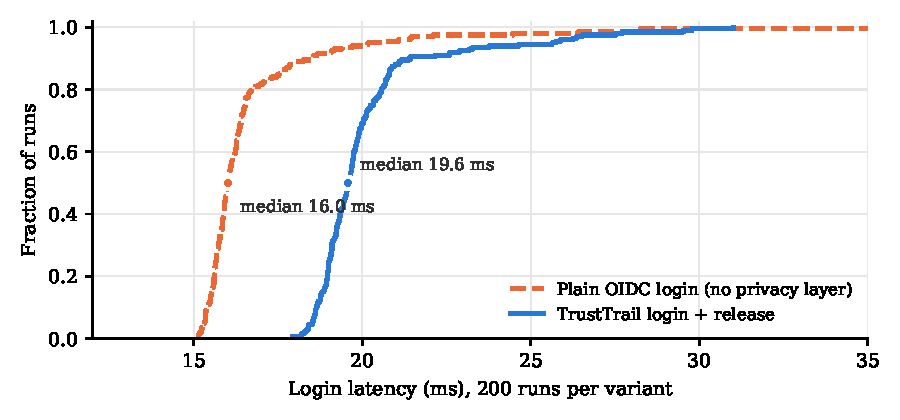
\includegraphics[width=0.85\linewidth]{figures/latency_ecdf.pdf}
\caption{Cumulative distribution of login latency. The TrustTrail curve is shifted right by the \code{/release} call, a few milliseconds. One baseline run at 49.4\,ms lies beyond the plotted range.}
\label{fig:latency}
\end{figure}

\emph{Interpretation.} The privacy layer costs a few milliseconds per login, which a user will not notice next to network and page-load times. The release call covers token verification, the declaration and cap checks, a request to Keycloak for the student record, the ledger transaction and an ECDSA signature; we did not time these steps separately. Because everything ran on one machine without network latency, the absolute numbers are lower than a deployment would see; the overhead in a deployment would also include one extra network round trip from the service to TrustTrail. We did not measure behaviour under concurrent load; all database writes go through one lock, so throughput is an open question (Section~\ref{sec:discussion}).

\subsection{Tamper detection}
\label{sec:eval-tamper}
\emph{Method.} The tamper experiment models adversary A5, an insider with write access to the database file. In each of five repetitions, the harness makes sure the ledger has at least six entries, anchors all of them, adds one more release after the anchor, and records the entry hashes contained in all stored receipts, which stand for the receipts that students have downloaded. It then picks a random target release (not the first and not the newest) and runs six attacks, each on a fresh copy of the live database with the append-only triggers dropped:
\begin{enumerate}
\item[A.] change an entry's released attributes and leave its stored hash;
\item[B.] change an entry's purpose and recompute its hash;
\item[C.] delete the entry;
\item[D.] change the entry and recompute every later hash, so the chain is consistent again;
\item[E.] cut off the tail of the ledger, from the last anchored entry onward;
\item[F.] change the release made after the last anchor and fix the hashes from there on.
\end{enumerate}
After each attack, three independent checks run: the hash chain verification, a check of every held receipt against the ledger (entry present and recomputed hash equal to the hash in the receipt), and verification of the ledger against the on-chain batches. The live ledger is never modified.

\emph{Results.} Table~\ref{tab:tamper} shows that every attack was detected by at least one check in all five repetitions, and every cell matched the outcome the design predicts. The hash chain alone missed attacks D, E and F, as Section~\ref{sec:design-ledger} explains. Receipts caught all six, because each attack changed or removed an entry for which a receipt exists. Anchoring caught all attacks on anchored entries, including D and E, which are invisible to the chain, but not attack F, which edits an entry made after the last anchor.

\begin{table}[t]
\centering
\caption{Tamper detection: repetitions in which each check detected the attack (of 5)}
\label{tab:tamper}
\small
\begin{tabular}{@{}lcccc@{}}
\toprule
Attack & Hash chain & Student receipts & Blockchain anchor & Any check \\
\midrule
A. change an entry, leave its hash & 5/5 & 5/5 & 5/5 & 5/5 \\
B. change an entry, recompute its hash & 5/5 & 5/5 & 5/5 & 5/5 \\
C. delete an entry & 5/5 & 5/5 & 5/5 & 5/5 \\
D. change an entry, recompute every later hash & 0/5 & 5/5 & 5/5 & 5/5 \\
E. cut off the tail of the ledger & 0/5 & 5/5 & 5/5 & 5/5 \\
F. change an entry made after the last anchor & 0/5 & 5/5 & 0/5 & 5/5 \\
\bottomrule
\end{tabular}
\end{table}

\emph{Interpretation.} The three mechanisms cover each other's gaps. The chain catches careless edits cheaply and locates them. Anchors catch every rewrite of anchored history, including a complete rewrite by the operator, for every student, whether or not that student kept a receipt. Receipts protect an individual student's own entries, including during the anchoring window. The one case where only receipts help, attack F, lasts at most one anchoring interval. The receipt result is optimistic in one respect: the experiment assumes students hold receipts for all affected entries, whereas in practice only students who download them do. The dashboard's own receipt check uses receipts stored by TrustTrail, which an attacker who also rewrote the receipts table would pass; only downloaded receipts are independent.

\subsection{Violation detection and trust response}
\label{sec:eval-violation}
\emph{Method.} The violation experiment models adversaries A1 and A2 with the three scripted services of Section~\ref{sec:implementation}. Each of three repetitions starts by resetting every service to its base tier (the resets are recorded in the ledger). Honest traffic comes first: each honest service receives releases for all five students twice, 30 releases per repetition. Then each bad service misbehaves five times. After each attempt the harness triggers a trust synchronisation and waits until the violation count changes, at most 15\,s, then records the score, tier and cap. An attempt counts as detected if a violation entry with the expected rule appears; a violation with another rule counts as a wrong rule; a violation recorded for an honest service is a false positive.

\emph{Results.} Table~\ref{tab:violations} shows that all 45 attempts were detected with the correct rule. Each first violation lowered the service by one tier, and the tier fell to \emph{blocked} by the second violation for the semi-trusted services and by the first for the untrusted one, after which the service could obtain only the anonymous profile. The 90 honest releases produced no violations and no tier changes. Rule~3 at login, which depends on reading Keycloak's event log, was detected as reliably as the synchronous rules.

\begin{table}[t]
\centering
\caption{Violation detection: three repetitions of five attempts per scripted service}
\label{tab:violations}
\small
\begin{tabularx}{\linewidth}{@{}l >{\raggedright\arraybackslash}X c c >{\raggedright\arraybackslash}p{4.6cm}@{}}
\toprule
Service & Misbehaviour (rule) & Detected & Wrong rule & Tier after attempts 1--5 \\
\midrule
Campus Deals & asks for attributes its declaration does not cover (1) & 15/15 & 0 & semi\_trusted $\rightarrow$ untrusted $\rightarrow$ blocked, stays blocked \\
Alumni Tracker & asks again after its deletion time (2) & 15/15 & 0 & semi\_trusted $\rightarrow$ untrusted $\rightarrow$ blocked, stays blocked \\
Career Portal & asks Keycloak for a profile above its cap (3) & 15/15 & 0 & untrusted $\rightarrow$ blocked, stays blocked \\
\midrule
Honest services & 90 releases & \multicolumn{2}{c}{0 false positives} & no tier changes \\
\bottomrule
\end{tabularx}
\end{table}

\emph{Interpretation.} The rules fire as designed and the feedback loop works: a service that breaks its promise twice is reduced to the anonymous profile within seconds, without human action, both at Keycloak and at release. The Alumni Tracker reaches \emph{blocked} after the same number of violations as Campus Deals although it starts at 85 points, because a score of 60 after one violation still means only one demotion. The 100\% detection rate is a property of scripted clients that misbehave in exactly the ways the rules describe. It does not estimate how often real services misbehave, and it says nothing about misuse after data has left TrustTrail.

\subsection{Anchoring cost and delay}
\label{sec:eval-anchoring}
\emph{Method.} The anchoring script produces a release about every 2\,s and triggers an anchor every 12\,s, for three batches, and records gas per transaction and the delay from each entry's timestamp to the confirmation of the transaction that anchors it. The contract tests measure the gas of the first anchor on a new contract and of an anchor covering a range of 100{,}000 entries.

\emph{Results.} Every anchor after the first cost 77{,}268 gas, whether it covered 6 entries, 7 entries or a range of 100{,}000 (Table~\ref{tab:gas}). The first anchor on a new contract cost 91{,}659 gas, because it initialises the batch array's storage, and deploying the contract cost 361{,}072 gas. With the 12\,s interval, the delay from entry to anchor had a median of 7.6\,s and a maximum of 12.8\,s over 19 entries; transactions were confirmed in at most 0.05\,s on the local chain.

\begin{table}[t]
\centering
\caption{Gas cost of anchoring on the local chain (10 November 2026)}
\label{tab:gas}
\small
\begin{tabular}{@{}lrr@{}}
\toprule
Operation & Entries covered & Gas \\
\midrule
Deploy \code{TrustTrailAnchor} & -- & 361{,}072 \\
First anchor on a new contract & -- & 91{,}659 \\
Later anchor (three measured batches) & 6, 6, 7 & 77{,}268 each \\
Later anchor (contract test) & 100{,}000 & 77{,}268 \\
\bottomrule
\end{tabular}
\end{table}

\emph{Interpretation.} The cost of anchoring is constant per batch, because the contract stores one 32-byte root and three numbers whatever the batch size. On a public chain the cost per batch is 77{,}268 gas multiplied by the gas price; at 1\,gwei, one anchor costs about 0.000077\,ETH, and a day of continuous traffic at the default 300\,s interval (288 anchors) about 0.022\,ETH. When nothing new is recorded, no transaction is sent. The delay scales with the interval: with the default of 300\,s, an entry waits on average about half the interval and at most one interval plus the block time, roughly 150\,s and 310\,s on a public network. These figures for a public chain are estimates from the local measurements; we did not run on Sepolia.

\subsection{Comparison with the base survey's taxonomy}
\label{sec:eval-taxonomy}
Table~\ref{tab:taxonomy} places TrustTrail in the taxonomy of Werner et al.~\cite{werner2017survey}, next to the four works in progress from the survey's Table~3. The marks for the four works are copied from the survey. The marks for TrustTrail are our own assessment, with the evidence from this paper; an assessment by authors of their own system is not independent, and we plan to have it repeated by someone who did not build TrustTrail.

\begin{table}[t]
\centering
\caption{TrustTrail and the authors' works in progress on the nine characteristics of~\cite{werner2017survey}. W1 = Weingärtner (survey ref.~[83]), W2 = Werner et al.~\cite{werner2015approach}, W3 = Bodnar et al.\ (survey ref.~[24]), W4 = Werner et al.~\cite{werner2016model}. Marks for W1--W4 are copied from the survey's Table~3 (``\checkmark'' = marked, ``p'' = partial). TrustTrail's marks are our self-assessment.}
\label{tab:taxonomy}
\small
\begin{tabularx}{\linewidth}{@{}l c c c c c >{\raggedright\arraybackslash}X@{}}
\toprule
Characteristic & W1 & W2 & W3 & W4 & TrustTrail & Evidence for TrustTrail \\
\midrule
Transparency & \checkmark & \checkmark & \checkmark & \checkmark & \checkmark & declared purpose and deletion date; dashboard lists every release and violation \\
Controllability & \checkmark & & \checkmark & \checkmark & -- & profiles set by tier, not chosen by the student; per-attribute choice only in a prototype \\
Minimization & & & & \checkmark & \checkmark & profile caps; tokens carry no claims; release = declared $\cap$ allowed \\
Accountability & & & & & \checkmark & signed declarations and receipts; hash chain; anchoring; Table~\ref{tab:tamper} \\
Data quality & \checkmark & & & & -- & IdP treated as the system of record \\
Use limitation & & & & & p & purpose and deletion date checked at every release; use after release not enforceable \\
User-friendly & & p & p & p & p & dashboard and receipts; not yet evaluated with users \\
Trust & \checkmark & & & \checkmark & p & behaviour-driven score and tier; heuristic weights \\
Obfuscation & & & & \checkmark & p & pairwise \code{sub} and no \code{sid}; anonymous profile still has a pairwise \code{sub} in the ID token \\
\bottomrule
\end{tabularx}
\end{table}

The comparison shows where TrustTrail adds to the survey's line of work: accountability and use limitation, which none of the four works address, and a trust level that follows observed behaviour. It also shows what TrustTrail gives up. The authors' works let the user choose a profile at each interaction, which counts towards controllability. TrustTrail decides the profile by the service's tier and the declaration; the student does not choose per release in the running system. Our usability-study prototype adds per-attribute choice to a consent screen, but it is not part of the evaluated system (Section~\ref{sec:future}).

\subsection{Answers to the research questions}
\begin{itemize}
\item \textbf{RQ1} (profiles and linkage): yes, with standard OIDC on the service side. Each service received only its profile's attributes, different pseudonyms, and no session identifier (Section~\ref{sec:eval-functional}); one custom Keycloak mapper was needed for the last property.
\item \textbf{RQ2} (purpose binding): yes. No release happens without a declaration signed by the service, requests outside it or after its deletion date are refused and recorded, and each release has a receipt bound to the declaration's hash.
\item \textbf{RQ3} (tamper evidence): yes, for all six attacks tried, including a full rewrite and truncation by the operator, with only hashes on chain (Table~\ref{tab:tamper}); entries newer than the last anchor rely on receipts.
\item \textbf{RQ4} (trust feedback): yes for the three observable rules; every scripted violation was detected and demoted the service, with no false positives (Table~\ref{tab:violations}).
\item \textbf{RQ5} (cost): a median of 3.6\,ms per login, and 77{,}268 gas per anchor regardless of batch size.
\end{itemize}

\subsection{Threats to validity}
\emph{Internal validity.} The latency benchmark uses the password grant, which skips the browser redirects; both variants skip them equally, but the TrustTrail variant's token request also differs slightly from the baseline's (pairwise identifier, mapper, no claim mappers). The tamper and violation experiments use attacks and clients that we wrote, and the expected outcomes were fixed in advance by the same team. \emph{External validity.} All measurements come from one laptop with local containers, invented data, five students and six services. A deployment adds network latency, more users and concurrent load. The local chain confirms transactions immediately; a public chain does not. \emph{Construct validity.} The taxonomy marks for TrustTrail are a self-assessment, and the survey's characteristics are broad enough that reasonable assessors could disagree, especially about controllability and trust.
